\chapter{Probing Results}
\label{chap:results}

\begin{figure}%[hb!]
    \centering
    \makebox[\textwidth][c]{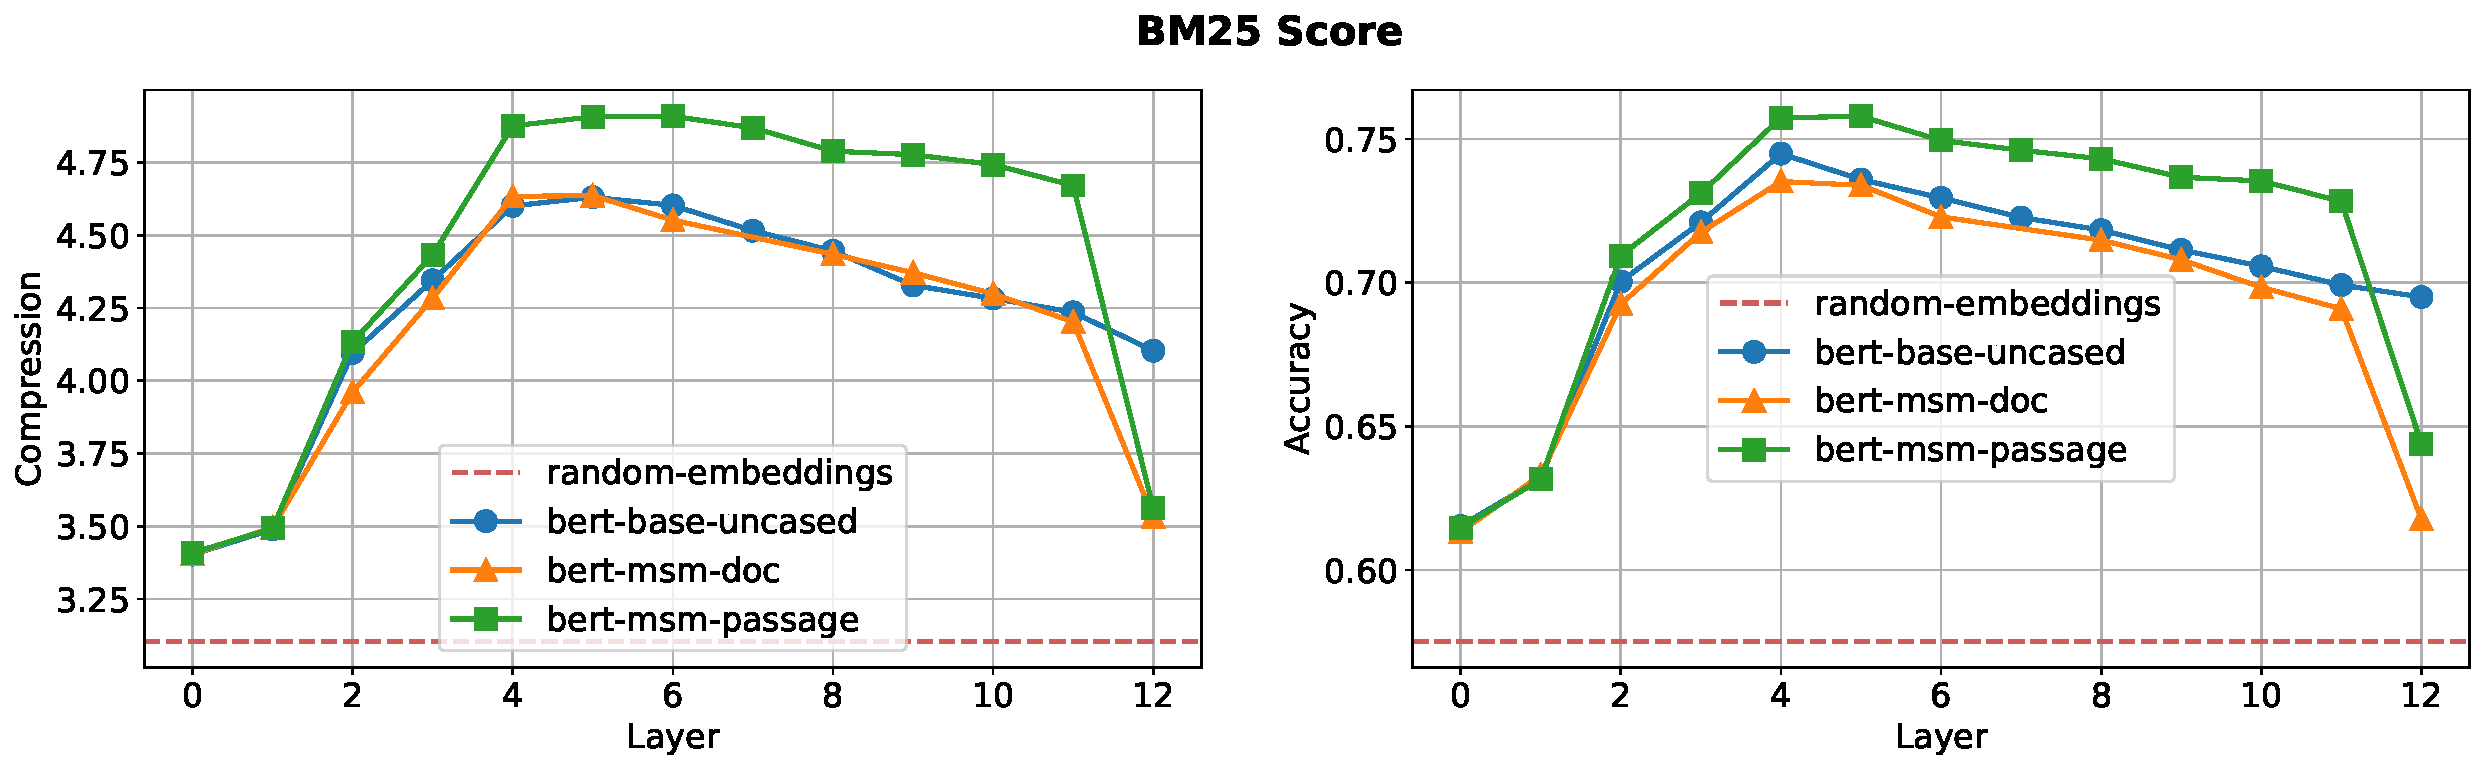
\includegraphics[width=1.25\textwidth]{gfx/probing/bm25}}
    \caption{\dots}
\end{figure}

\begin{figure}
    \centering
    \makebox[\textwidth][c]{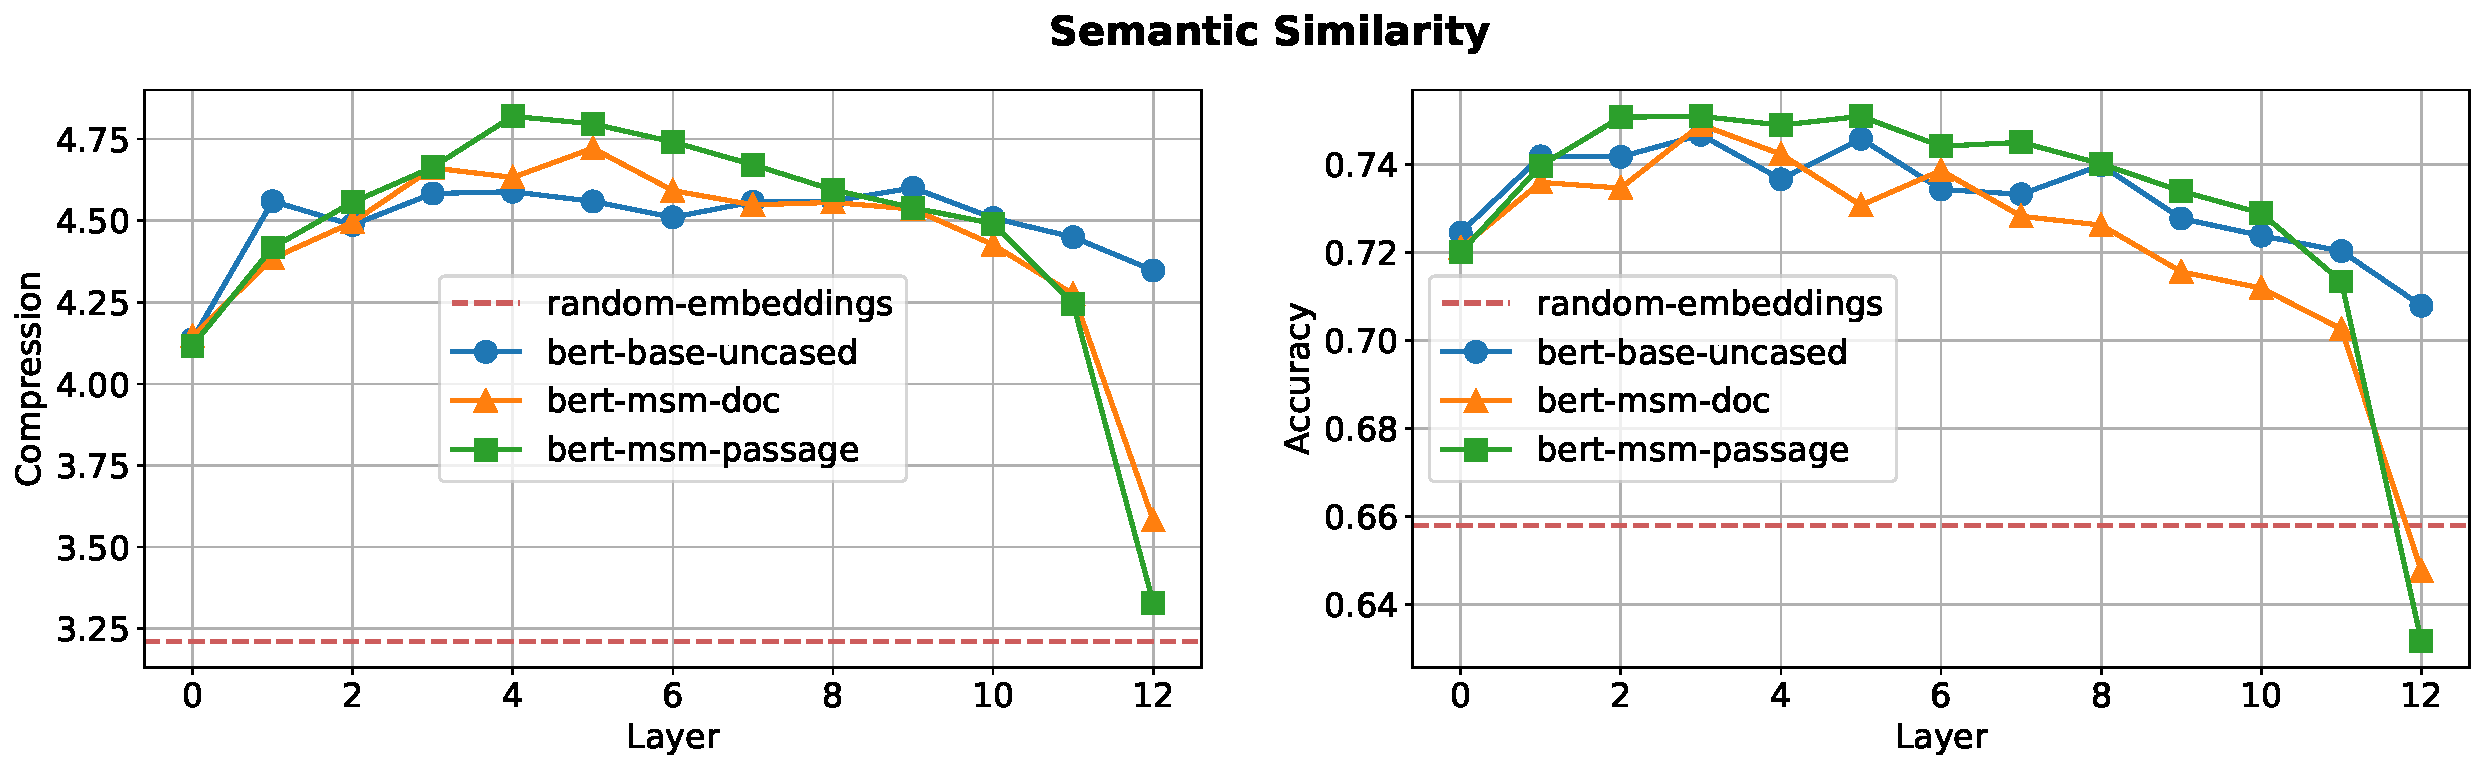
\includegraphics[width=1.25\textwidth]{gfx/probing/sem_sim}}
    \caption{\dots }
\end{figure}

\begin{figure}
    \centering
    \makebox[\textwidth][c]{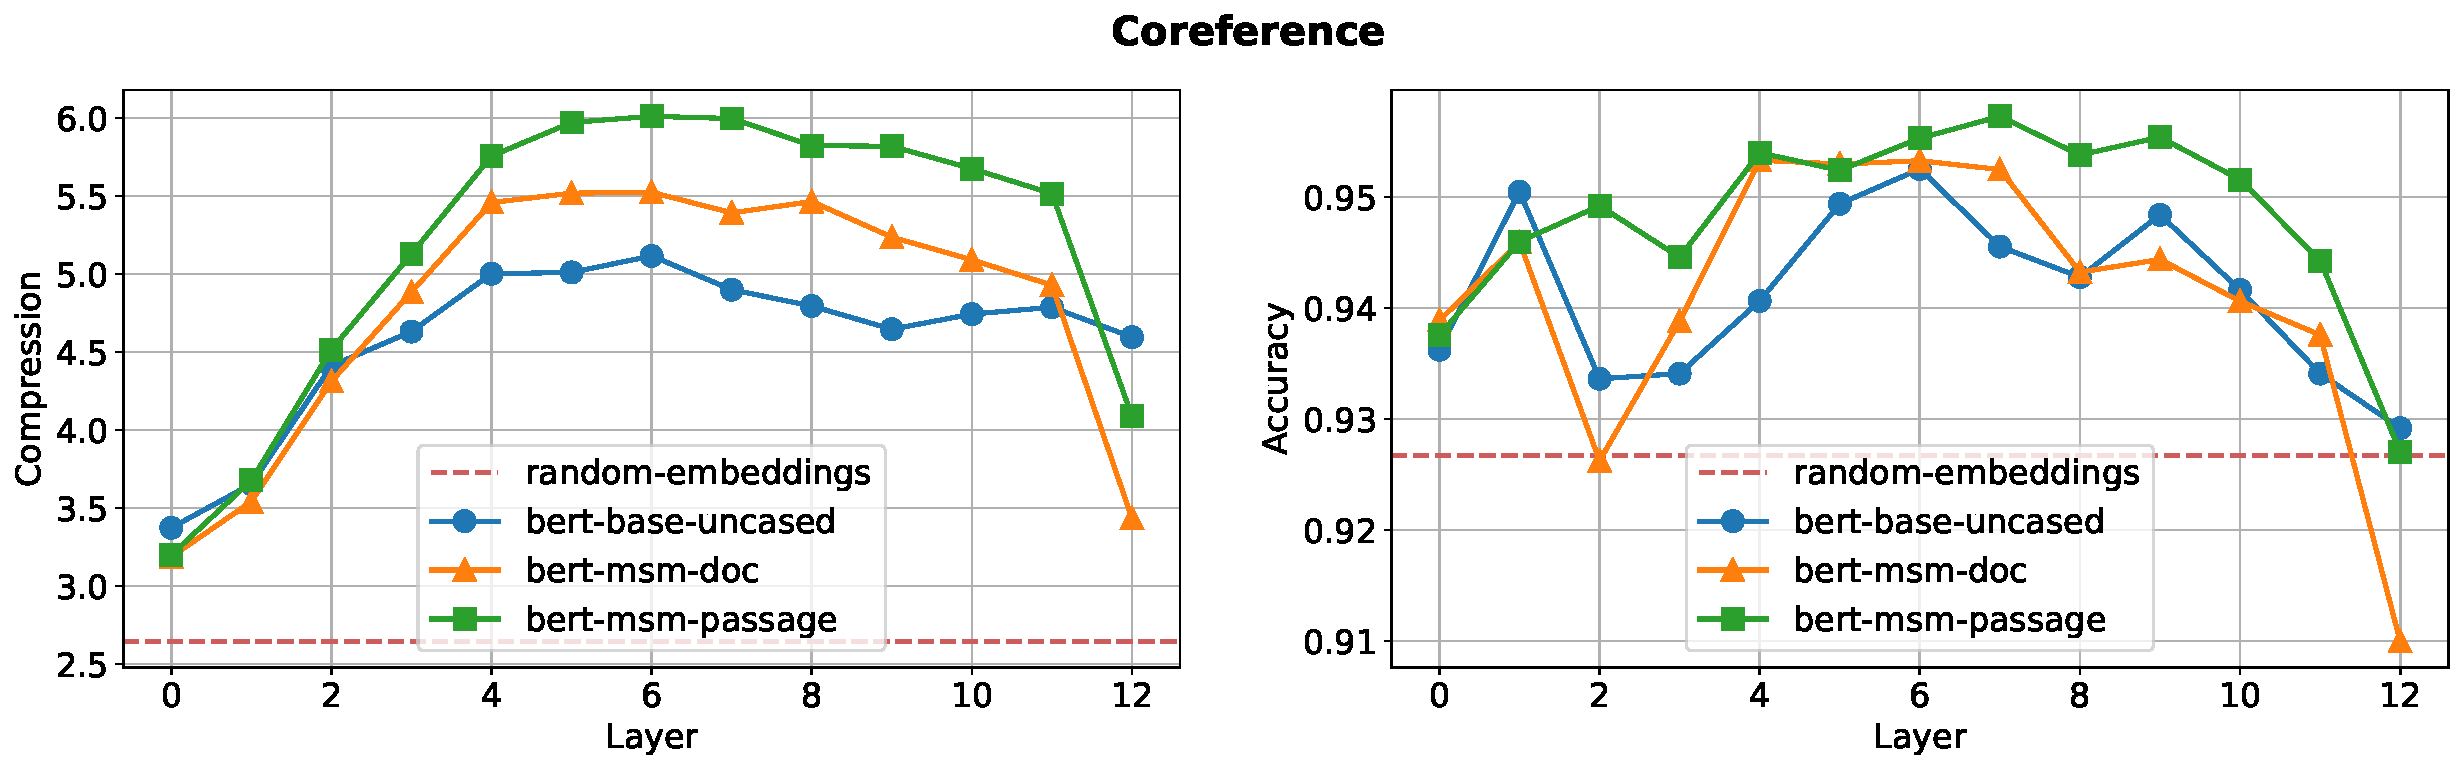
\includegraphics[width=1.25\textwidth]{gfx/probing/coref}}
    \caption{\dots}
\end{figure}


\begin{figure}
    \centering
    \makebox[\textwidth][c]{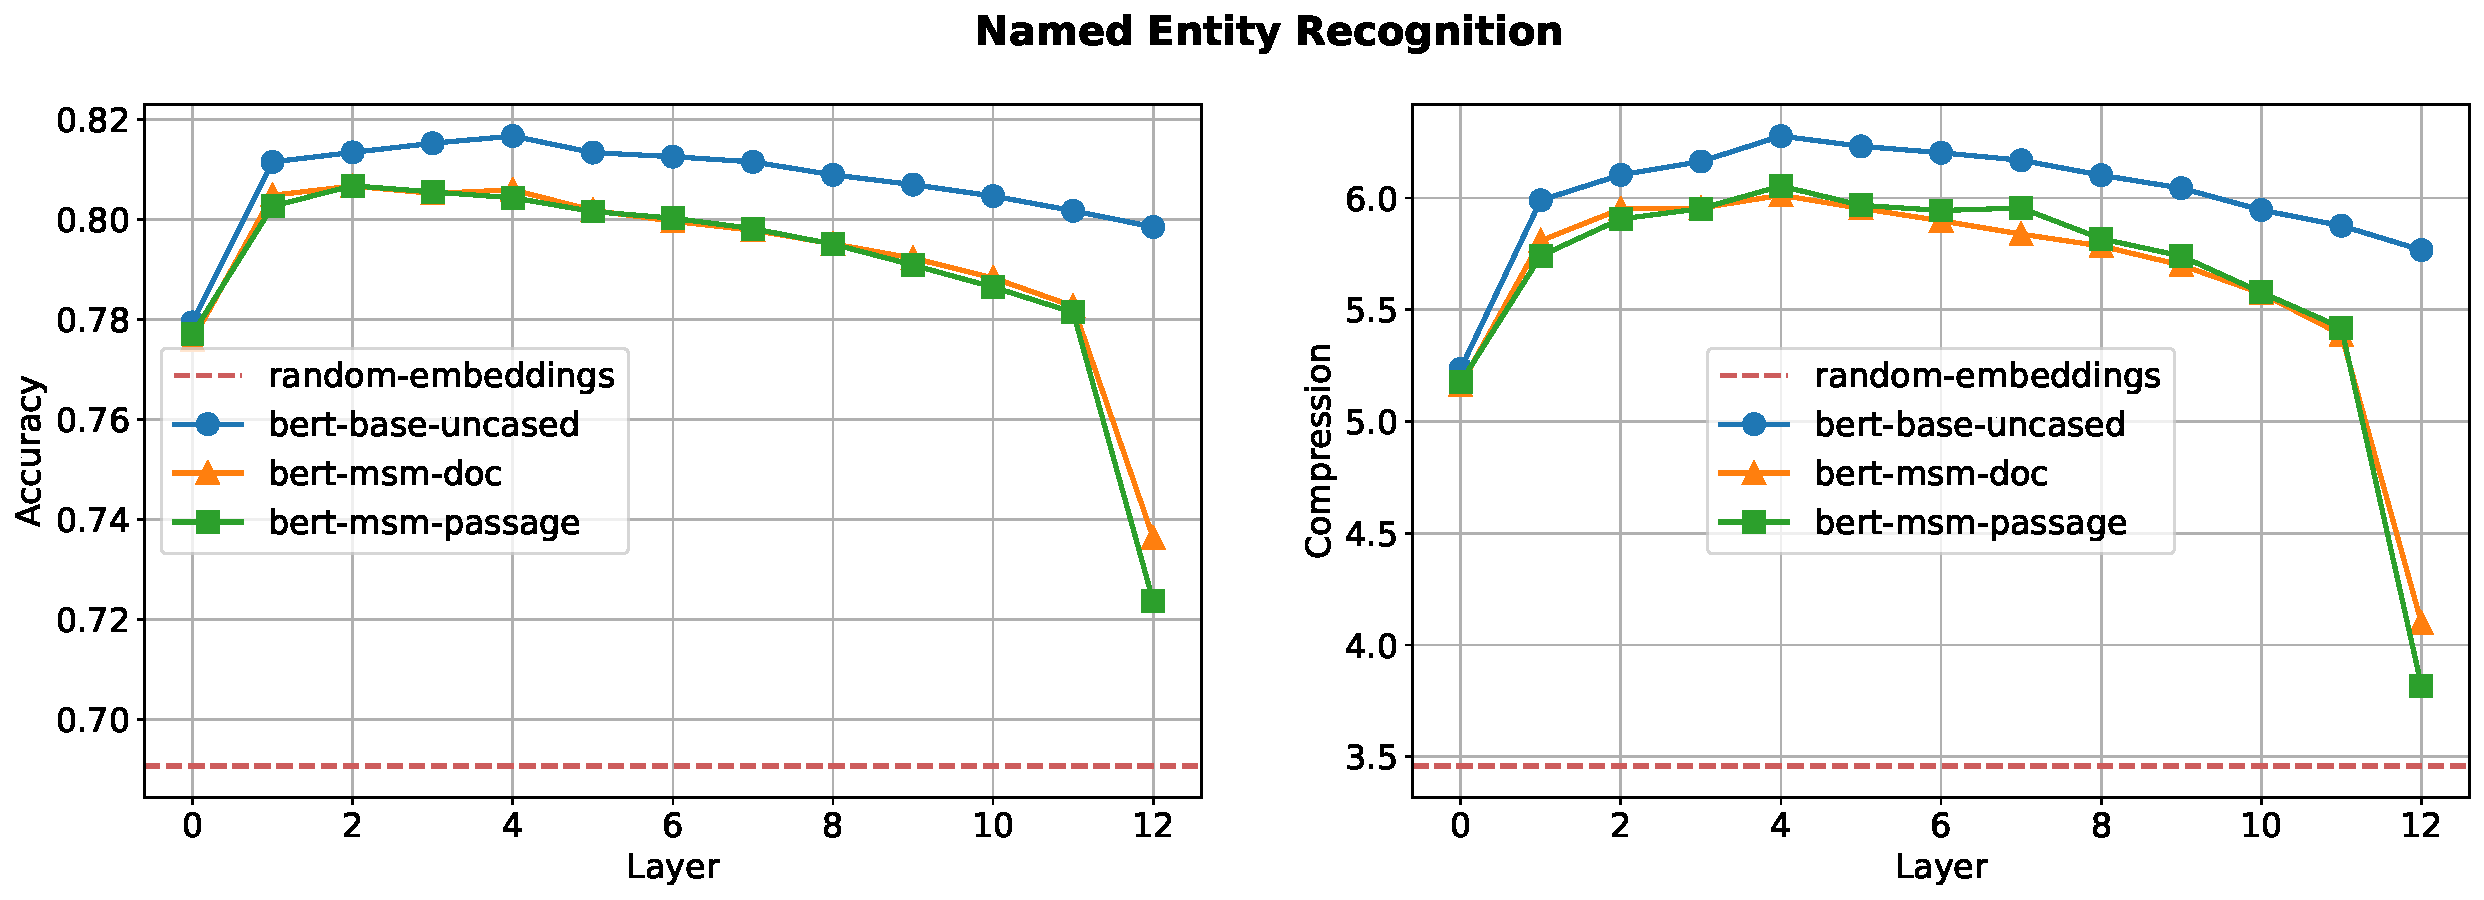
\includegraphics[width=1.25\textwidth]{gfx/probing/ner}}
    \caption{\dots}
\end{figure}

\begin{figure}
    \centering
    \makebox[\textwidth][c]{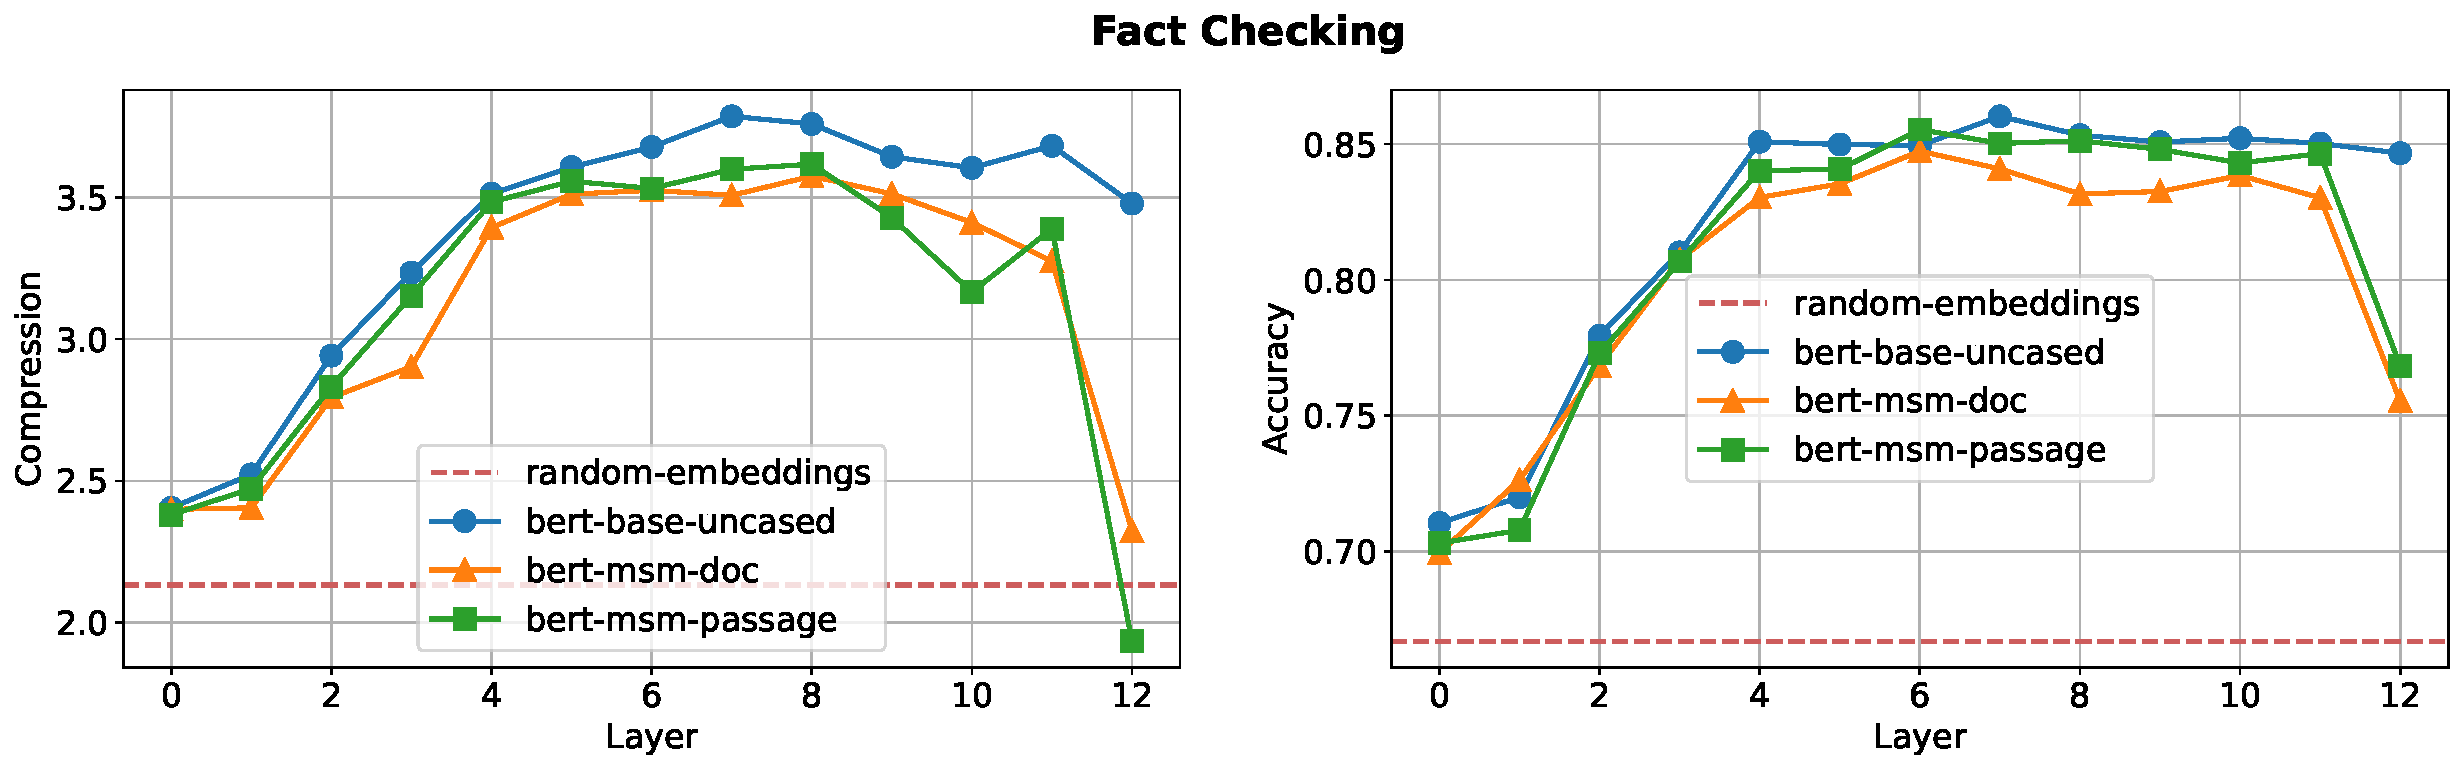
\includegraphics[width=1.25\textwidth]{gfx/probing/fact_check}}
    \caption{\dots}
\end{figure}



\begin{figure}
    \centering
    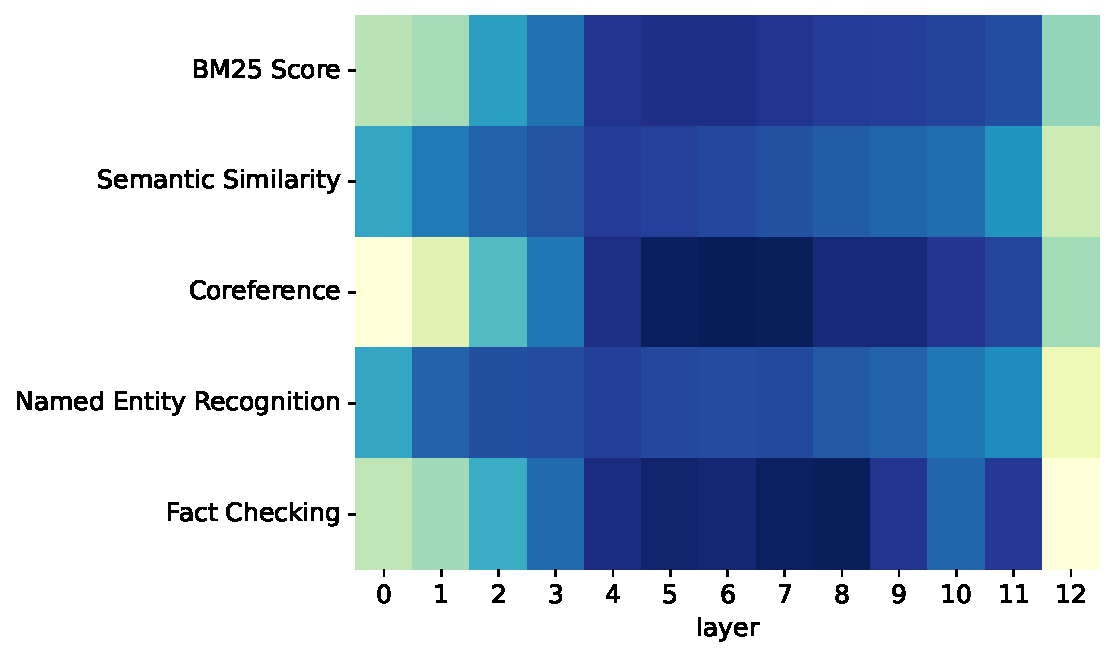
\includegraphics[width=\textwidth]{gfx/probing/heatmap_compression}
    \caption{Compression as a function of task and layer, row-normalized.}
\end{figure}

\begin{figure}
    \centering
    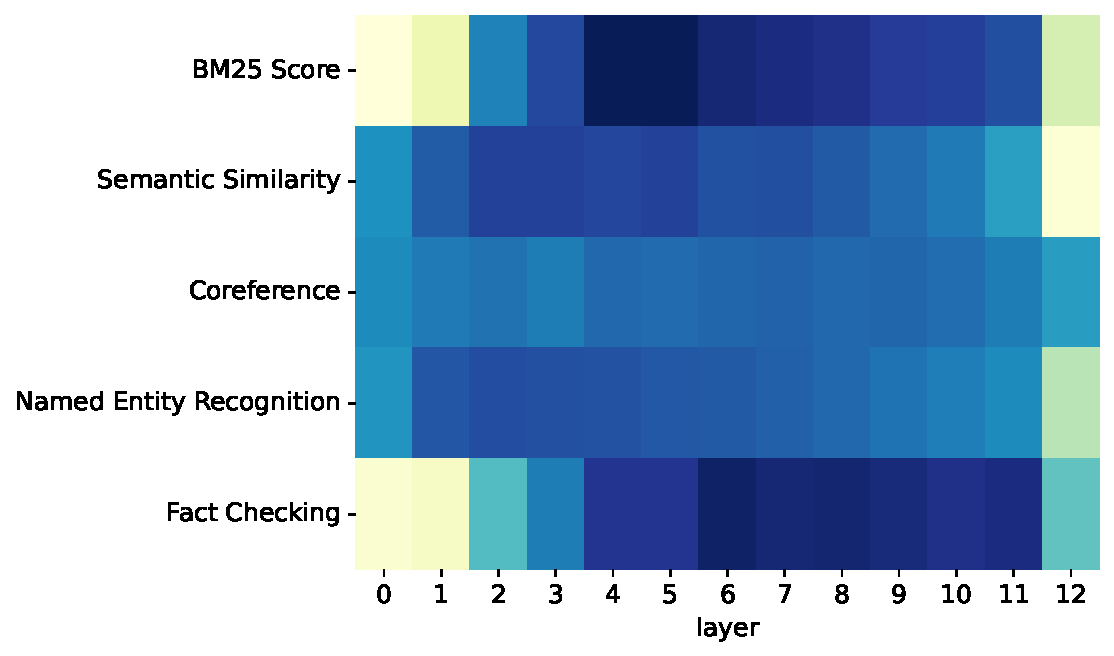
\includegraphics[width=\textwidth]{gfx/probing/heatmap_accuracy}
    \caption{Accuracy as a function of task and layer, row-normalized.}
\end{figure}

\begin{figure}
    \centering
    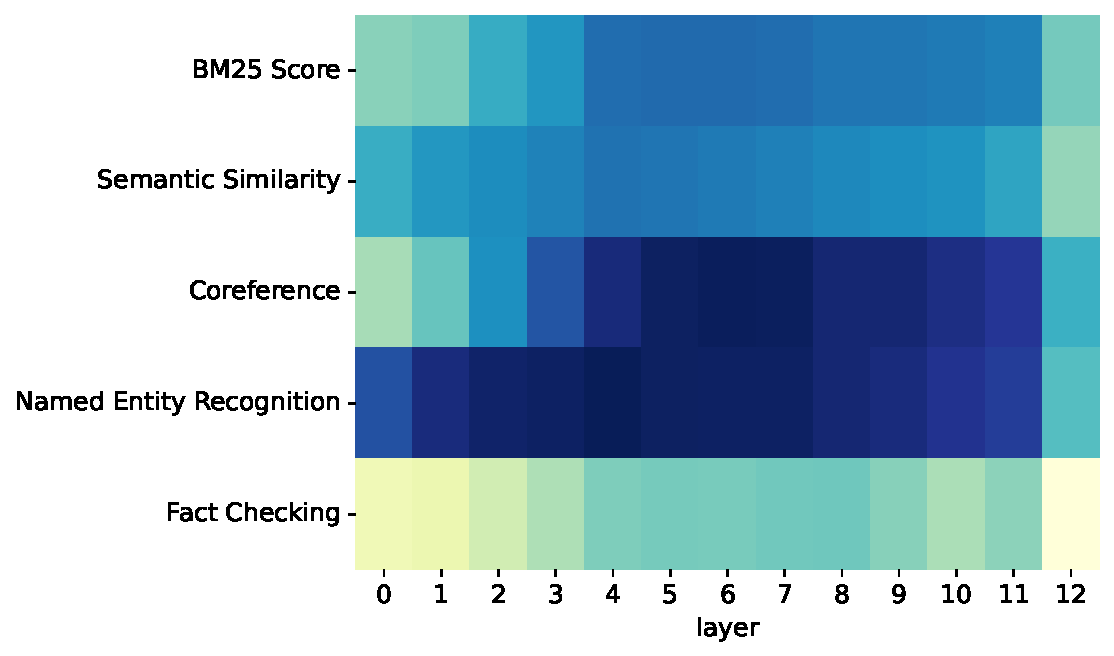
\includegraphics[width=\textwidth]{gfx/probing/abs_heatmap_compression}
    \caption{Compression as a function of task and layer, absolute values.}
\end{figure}
